\documentclass[12pt]{article}
\usepackage[utf8]{inputenc}
\usepackage[a4paper, total={6.5in, 9.5in}]{geometry}
\usepackage{authblk}
\usepackage{multirow}
\usepackage{graphicx}
\usepackage{amsmath}
\usepackage{biblatex}
\usepackage{rotating}
\usepackage{ragged2e}
\usepackage{multicol}
\usepackage{float}
\usepackage{algpseudocode}
\usepackage{enumitem}
\usepackage{caption}
\usepackage{subcaption}
\usepackage{hyperref}
\hypersetup{
    colorlinks=true,
    linkcolor=blue,
    }
\usepackage[label=corner]{karnaugh-map}
\usepackage[siunitx, RPvoltages]{circuitikz}
\usetikzlibrary{calc}
\usepackage{tikz}
\usetikzlibrary{positioning, shapes, arrows.meta, calc}

\title{CSE 306 \\
Computer Architecture Sessional \\
\vspace{10mm}
Assignment-2: 32-bit Floating Point Adder Simulation \\
\vspace{20mm}
Section - A1 \\
Group - 01 \\
\vspace{15mm}
\RaggedRight
Members of the Group: \\
\normalsize	{
\begin{enumerate}[label=\roman*]
    \item 1905001 - Mohammad Sadat Hossain
    \item 1905002 - Nafis Tahmid
    \item 1905004 - Asif Azad
    \item 1905005 - Md. Ashrafur Rahman Khan
    \item 1905008 - Shattik Islam Rhythm
\end{enumerate}
}
}
\author{}
\date{}

\begin{document}

\maketitle

\newpage
\section{\large{Introduction}}
A floating point number is a representation of a real number in a computer, with a fixed number of digits before and after the decimal point. A floating point adder is the digital circuit that performs addition and subtraction on floating point numbers.  It may be used to represent numbers that are too large or too small to be represented accurately with integer representations.\\
\newline
The floating point representation of a number consists of three fields: the sign bit, the exponent field, and the mantissa field. The sign bit represents the sign, either positive or negative. The exponent field allows the significand to be multiplied by a power of the base, using a fixed number of bits in a biased form, in order to represent a wide range of values. To obtain the actual exponent, the bias has to be subtracted from the stored bits. The mantissa is the fractional part of the number, containing the digits after the decimal point.  In this implementation, the sign bit, the exponent field and the mantissa take up 1, 12 and 19 bits respectively. Thus, the exponent bias for our problem would be $2^{12-1} - 1 = 2047$.\\
\newline
A floating point adder works by aligning the decimal points of the two numbers to be added and then adding the mantissas. The exponent of the result is fixed making required shifts and corresponding adjustments(increment/decrement) going through the process of normalization and rounding. The sign of the result is based on the signs of the two numbers being added.\\
\newline
Floating point adder is used in a variety of applications, including scientific and engineering calculations, financial modeling, and computer graphics. It is used in co-processors to perform fast, hardware-accelerated floating point arithmetic as they can be computationally intensive. A dedicated floating point adder can perform these calculations much faster than the main processor. This can be especially important in applications such as scientific simulations, data analysis, and other tasks that require high-precision floating point calculations.\\


\section{\large{Problem Specification}}
The assignment asks to design a floating point adder circuit which takes two floating points as inputs and provides their sum, another floating point as output. Each floating point will be 32 bits long with the following representation:
\begin{table}[H]
    \centering
    \begin{tabular}{|p{3cm}|p{3cm}|p{3cm}|}
        \hline
         \large{\textbf{Sign}}&\large{\textbf{Exponent}}&\large{\textbf{Fraction}}  \\
         \hline
         {1 bit}&{12 bits}&{19 bits} \\
         \hline
    \end{tabular}
    \caption{Problem Specification}
    \label{tab:spec}
\end{table}
\newpage

\section{\large{Description and Circuit Diagram of Modules}}
Several libraries have been implemented for the sake of modularity in the design of the floating point adder. Descriptions and usages of the libraries are given below:

\subsection{Multiplexer Library}
Multiplexer library(MuxLib.circ) has several circuits to help with multiplexing in the floating point adder. The important components are:
\begin{itemize}
    \item Abstracted 4 bit 2 to 1 Mux (This circuit abstracts the IC 74157 for ease of use) [4Mux2X1]
    \item 4 bit 4 to 1 Mux [4Mux4X1]
    \item 12 bit 2 to 1 Mux [12Mux2X1]
    \item 32 bit 2 to 1 Mux [32Mux2X1]
    \item 32 bit 4 to 1 Mux [32Mux4X1]
\end{itemize}
\begin{figure}[H]
    \centering
    \begin{subfigure}[b]{0.3\textwidth}
        \includegraphics[width=\textwidth]{Images/4MUX2X1.png}
        \caption{4 bit $2\times1$ MUX}
        \label{fig:4b2x1mux}
    \end{subfigure}
    \begin{subfigure}[b]{0.3\textwidth}
        \includegraphics[width=\textwidth]{Images/4MUX4X1.png}
        \caption{4 bit $4\times1$ MUX}
        \label{fig:4b4x1mux}
    \end{subfigure}
    \begin{subfigure}[b]{0.3\textwidth}
        \includegraphics[width=\textwidth]{Images/12MUX2X1.png}
        \caption{12 bit $2\times1$ MUX}
        \label{fig:12b2x1}
    \end{subfigure}
    \newline
    \newline
    \begin{subfigure}[b]{0.45\textwidth}
        \includegraphics[width=\textwidth]{Images/32MUX2X1.png}
        \caption{32 bit $2\times1$ MUX}
        \label{fig:32b2x1}
    \end{subfigure}
    \begin{subfigure}[b]{0.45\textwidth}
        \includegraphics[width=\textwidth]{Images/32MUX4X1.png}
        \caption{32 bit $4\times1$ MUX}
        \label{fig:32b4x1}
    \end{subfigure}
    \caption{Multiplexer Circuits}\label{fig:mux}
\end{figure}

\subsection{Comparator Library}
To compare the exponenets of the inputs, a 12 bit comparator is constructed using IC 7485. This library(ComparatorLib.circ) holds the circuit 12BitMagnitudeComparator which takes two 12 bit numbers and compare them.
\begin{figure}[H]
    \centering
        \includegraphics[width=\textwidth]{Images/12BitMagnitudeComparator.png}
        \label{fig:12bitmagcomp}
    \caption{12 Bit Magnitude Comparator}
\end{figure}

\subsection{Adder Library}
In floating point adder, we need adders and subtractors in several places. To make the work easier, an adder library(AdderLib.circ) is constructed. It includes:
\begin{itemize}
    \item 4, 12, 32 bit adder [4Adder, 12Adder, 32Adder]
    \item 4, 12, 32 bit 1's complementer [1Compl4, 1Compl12, 1Compl32]
    \item 12, 32 bit 2's complementer [2Compl12, 2Compl32]
    \item 12 bit subtractor [12Sub]
\end{itemize}
\begin{figure}[H]
    \centering
    \begin{subfigure}[b]{0.3\textwidth}
        \includegraphics[width=\textwidth]{Images/4Adder.png}
        \caption{4 Bit Adder}
        \label{fig:4bitadder}
    \end{subfigure}
    \begin{subfigure}[b]{0.3\textwidth}
        \includegraphics[width=\textwidth]{Images/12Adder.png}
        \caption{12 Bit Adder}
        \label{fig:12bitadder}
    \end{subfigure}
    \begin{subfigure}[b]{0.3\textwidth}
        \includegraphics[width=\textwidth]{Images/32Adder.png}
        \caption{32 Bit Adder}
        \label{fig:32bitadder}
    \end{subfigure}
    \newline
    \newline
    \begin{subfigure}[b]{0.3\textwidth}
        \includegraphics[width=\textwidth]{Images/1Compl4.png}
        \caption{4 Bit 1's Complementer}
        \label{fig:4bitcompl}
    \end{subfigure}
    \begin{subfigure}[b]{0.3\textwidth}
        \includegraphics[width=\textwidth]{Images/1Compl12.png}
        \caption{12 Bit 1's Complementer}
        \label{fig:12bitcompl}
    \end{subfigure}
    \begin{subfigure}[b]{0.3\textwidth}
        \includegraphics[width=\textwidth]{Images/1Compl32.png}
        \caption{32 Bit 1's Complementer}
        \label{fig:32bitcompl}
    \end{subfigure}
    \newline
    \newline
    \begin{subfigure}[b]{0.3\textwidth}
        \includegraphics[width=\textwidth]{Images/2Compl12.png}
        \caption{12 Bit 2's Complementer}
        \label{fig:12bit2compl}
    \end{subfigure}
    \begin{subfigure}[b]{0.3\textwidth}
        \includegraphics[width=\textwidth]{Images/2Compl32.png}
        \caption{32 Bit 2's Complementer}
        \label{fig:32bit2compl}
    \end{subfigure}
    \begin{subfigure}[b]{0.3\textwidth}
        \includegraphics[width=\textwidth]{Images/12Sub.png}
        \caption{12 Bit Subtractor}
        \label{fig:12bitsub}
    \end{subfigure}
    \caption{Adder Circuits}\label{fig:adder}
\end{figure}


\subsection{Shifter Library}
In floating point adder we need shifters to shift the fraction in order to balance with the other operand or normalize. We have implemented shifters(ShiftLib.circ) with splitters and muxes implemented in multiplexer library. The circuits in the library are:
\begin{itemize}
    \item 1, 2, 4, 8, 16 bits left shifter [1LeftShift, 2LeftShift, 4LeftShift, 8LeftShift, 16LeftShift]
    \item 1, 2, 4, 8, 16 bits right shifter [1RightShift, 2RightShift, 4RightShift, 8RightShift, 16RightShift]
    \item Arbitrary left and right shifter (Can shift any number of bits up to 31 bits) [ArbLeftShift, ArbRightShift]
    \item Right shifter that will make every bit 0 if it needs shfting more than 31 bits [RightShiftWithEmpty]
\end{itemize}
\begin{figure}[H]
    \centering
    \begin{subfigure}[b]{0.3\textwidth}
        \includegraphics[width=\textwidth]{Images/1LeftShift.png}
        \caption{1 Bit Left Shifter}
        \label{fig:1leftshift}
    \end{subfigure}
    \hfill
    \begin{subfigure}[b]{0.3\textwidth}
        \includegraphics[width=\textwidth]{Images/2LeftShift.png}
        \caption{2 Bit Left Shifter}
        \label{fig:2leftshift}
    \end{subfigure}
    \hfill
    \begin{subfigure}[b]{0.3\textwidth}
        \includegraphics[width=\textwidth]{Images/4LeftShift.png}
        \caption{4 Bit Left Shifter}
        \label{fig:4leftshift}
    \end{subfigure}
    \newline
    \newline
    \begin{subfigure}[b]{0.3\textwidth}
        \includegraphics[width=\textwidth]{Images/8LeftShift.png}
        \caption{8 Bit Left Shifter}
        \label{fig:8leftshift}
    \end{subfigure}
    \hfill
    \begin{subfigure}[b]{0.3\textwidth}
        \includegraphics[width=\textwidth]{Images/16LeftShift.png}
        \caption{16 Bit Left Shifter}
        \label{fig:16leftshift}
    \end{subfigure}
    \hfill
    \begin{subfigure}[b]{0.3\textwidth}
        \includegraphics[width=\textwidth]{Images/ArbLeftShift.png}
        \caption{Arbitrary Left Shifter}
        \label{fig:arbleftshift}
    \end{subfigure}
    \newline
    \newline
    \begin{subfigure}[b]{0.3\textwidth}
        \includegraphics[width=\textwidth]{Images/1RightShift.png}
        \caption{1 Bit Right Shifter}
        \label{fig:1rightshift}
    \end{subfigure}
    \hfill
    \begin{subfigure}[b]{0.3\textwidth}
        \includegraphics[width=\textwidth]{Images/2RightShift.png}
        \caption{2 Bit Right Shifter}
        \label{fig:2rightshift}
    \end{subfigure}
    \hfill
    \begin{subfigure}[b]{0.3\textwidth}
        \includegraphics[width=\textwidth]{Images/4RightShift.png}
        \caption{4 Bit Right Shifter}
        \label{fig:4rightshift}
    \end{subfigure}
    \newline
    \newline
    \begin{subfigure}[b]{0.3\textwidth}
        \includegraphics[width=\textwidth]{Images/8RightShift.png}
        \caption{8 Bit Right Shifter}
        \label{fig:8rightshift}
    \end{subfigure}
    \hfill
    \begin{subfigure}[b]{0.3\textwidth}
        \includegraphics[width=\textwidth]{Images/16RightShift.png}
        \caption{16 Bit Right Shifter}
        \label{fig:16rightshift}
    \end{subfigure}
    \hfill
    \begin{subfigure}[b]{0.3\textwidth}
        \includegraphics[width=\textwidth]{Images/ArbRightShift.png}
        \caption{Arbitrary Right Shifter}
        \label{fig:arbrightshift}
    \end{subfigure}
    \newline
    \newline
    \begin{subfigure}[b]{0.6\textwidth}
        \includegraphics[width=\textwidth]{Images/RightShiftWithEmpty.png}
        \caption{Right Shift With Empty}
        \label{fig:rightshiftwithempty}
    \end{subfigure}
    \caption{Shifter Circuits}\label{fig:shifter}
\end{figure}



\subsection{Encoder Library}
To normalize the final result, we need to locate the first set bit from left to right. It can be done easily using priority encoder. To help with this task, this library(EncoderLib.circ) is implemented. The contents of this library are:
\begin{itemize}
    \item 8 to 3 priority encoder (Constructed using 74147 IC) [8x3 Priority Encoder]
    \item 4 to 2 priority encoder (Constructed using 8 to 3 priority encoder of this library) [4x2 Priority Encoder]
    \item Circuit that finds the required number of bit shifts to normalize (Constructed using the aforementioned encoders) [ShiftFinder]
\end{itemize}
\begin{figure}[H]
    \centering
    \begin{subfigure}[b]{0.45\textwidth}
        \includegraphics[width=\textwidth]{Images/8X3PriorityEncoder.png}
        \caption{8$\times$3 Priority Encoder}
        \label{fig:8xprioenc}
    \end{subfigure}
    \begin{subfigure}[b]{0.45\textwidth}
        \includegraphics[width=\textwidth]{Images/4X2PriorityEncoder.png}
        \caption{4$\times$2 Priority Encoder}
        \label{fig:4x2prioenc}
    \end{subfigure}
    \newline
    \newline
    \begin{subfigure}[b]{0.9\textwidth}
        \includegraphics[width=\textwidth]{Images/ShiftFinder.png}
        \caption{Shift Finder}
        \label{fig:shiftfinder}
    \end{subfigure}
    \caption{Encoder Circuits}\label{fig:encoder}
\end{figure}

\subsection{Normalizer Library}
This library(NormalizerLib.circ) contains the circuit Normalization which normalizes the output with required number of bit shifts with the help of encoder library. Also it generates the 12 bit number which will be added to the exponent to complete normalization.
\begin{figure}[H]
    \centering
        \includegraphics[width=\textwidth]{Images/Normalization.png}
    \caption{Output Normalizer}\label{fig:normalizer}
\end{figure}

\subsection{Miscellaneous Library}
This library(MiscLib.circ) contains many circuits that helps to increase modularity and ease of implementation:
\begin{itemize}
    \item Bit extenders or bit extractors (20 to 32 bit, 19 to 32 bit, 5 to 12 bit, 32 to 19 bit) [20to32, 19to32, 5to12, 32to19]
    \item 0 checkers to see if all the bits are 0 [4Is0, 12Is0, 32Is0]
    \item Input processor that separates the different parts of floating point representation [InputProcess]
    \item Output processor that combines the different parts of floating point number [OutputProcess]
    \item Checker that checks whether there is an input with zero in exponenet [InputCheck]
    \item Circuit that changes the sign bit to 0, if any number representing zero is input with a 1 as sign bit [0handler]
    \item 4 bit OR, 32 bit OR [4OR, 32OR]
    \item Circuit that determines if rounding up is needed [Rounding]
\end{itemize}
\begin{figure}[H]
    \centering
    \begin{subfigure}[b]{0.45\textwidth}
        \includegraphics[width=\textwidth]{Images/20to32.png}
        \caption{20 to 32 Bit Extractor}
        \label{fig:20t32}
    \end{subfigure}
    \begin{subfigure}[b]{0.45\textwidth}
        \includegraphics[width=\textwidth]{Images/19to32.png}
        \caption{19 to 32 Bit Extractor}
        \label{fig:19t32}
    \end{subfigure}
    \newline
    \newline
    \begin{subfigure}[b]{0.45\textwidth}
        \includegraphics[width=\textwidth]{Images/5to12.png}
        \caption{5 to 12 Bit Extractor}
        \label{fig:5t12}
    \end{subfigure}
    \begin{subfigure}[b]{0.45\textwidth}
        \includegraphics[width=\textwidth]{Images/32to19.png}
        \caption{32 to 19 Bit Extractor}
        \label{fig:32t19}
    \end{subfigure}
    \caption{Bit Extractors}\label{fig:bitextract}
\end{figure}
\begin{figure}[H]
    \centering
    \begin{subfigure}[b]{0.3\textwidth}
        \includegraphics[width=\textwidth]{Images/4Is0.png}
        \caption{4 Bit Zero Checker}
        \label{fig:4is0}
    \end{subfigure}
    \begin{subfigure}[b]{0.3\textwidth}
        \includegraphics[width=\textwidth]{Images/12Is0.png}
        \caption{12 Bit Zero Checker}
        \label{fig:12is0}
    \end{subfigure}
    \begin{subfigure}[b]{0.3\textwidth}
        \includegraphics[width=\textwidth]{Images/32Is0.png}
        \caption{32 Bit Zero Checker}
        \label{fig:32is0}
    \end{subfigure}
    \caption{Zero Checkers}\label{fig:zerocheck}
\end{figure}
\begin{figure}[H]
    \centering
    \begin{subfigure}[b]{0.45\textwidth}
        \includegraphics[width=\textwidth]{Images/InputProcess.png}
        \caption{Input Processor}
        \label{fig:inpprocess}
    \end{subfigure}
    \begin{subfigure}[b]{0.45\textwidth}
        \includegraphics[width=\textwidth]{Images/OutputProcess.png}
        \caption{Output Processor}
        \label{fig:outprocess}
    \end{subfigure}
    \newline
    \newline
    \begin{subfigure}[b]{0.45\textwidth}
        \includegraphics[width=\textwidth]{Images/InputChecker.png}
        \caption{Input Checker}
        \label{fig:inpcheck}
    \end{subfigure}
    \begin{subfigure}[b]{0.45\textwidth}
        \includegraphics[width=\textwidth]{Images/0handler.png}
        \caption{Zero Handler}
        \label{fig:0handler}
    \end{subfigure}
    \caption{Input Output Processors}\label{fig:ioprocess}
\end{figure}
\begin{figure}[H]
\centering
 \begin{subfigure}[b]{0.3\textwidth}
  \includegraphics[width=\textwidth]{Images/4OR.png}
  \caption{4 Bit OR}
  \label{fig:4or}
  \end{subfigure}
  \begin{subfigure}[b]{0.3\textwidth}
  \includegraphics[width=\textwidth]{Images/32OR.png}
  \caption{32 Bit OR}
  \label{fig:32or}
  \end{subfigure}
  \begin{subfigure}[b]{0.3\textwidth}
  \includegraphics[width=\textwidth]{Images/Rounding.png}
  \caption{Rounding Determiner}
  \label{fig:rounddet}
 \end{subfigure}
 \caption{Other Useful Circuits}\label{fig:other}
\end{figure}

\newpage
\subsection{Rounding Circuit}
The name of this module is RoundingMachine.circ. It contains the circuit RoundingMachine that uses the Rounding circuit in the miscellaneous library and does the rounding of the mantissa.
\begin{figure}[H]
    \centering
        \includegraphics[width=\textwidth]{Images/Rounding.png}
    \caption{Rounder}\label{fig:rounder}
\end{figure}

\newpage
\subsection{Processing the Input}
This module(InputHandler.circ) helps to process the input for further operations in the floating point adder. It contains:
\begin{itemize}
    \item Exponent differentiator that calculates the difference between the exponenets of two inputs [ExpDiff12]
    \item A circuit that determines which input is greater than the other, greater exponent etc for control decisions [InputHandle]
\end{itemize}
\begin{figure}[H]
\centering
 \begin{subfigure}[b]{0.45\textwidth}
  \includegraphics[width=\textwidth]{Images/ExpDiff12.png}
  \caption{Exponent Differentiator}
  \label{fig:expdiff}
  \end{subfigure}
  \hfill
  \begin{subfigure}[b]{0.45\textwidth}
  \includegraphics[width=\textwidth]{Images/InputHandle.png}
  \caption{Input Handler}
  \label{fig:inphandle}
  \end{subfigure}
 \caption{Input Operator}\label{fig:inpproc}
\end{figure}



\newpage
\subsection{Adder Module}
This module(Added.circ) encapsulates all the works from taking input up to adding/subtracting. This module includes the circuit AddedInp which does this job.
\begin{figure}[H]
    \centering
        \includegraphics[width=0.85\textwidth]{Images/AddedInp.png}
    \caption{Adder}\label{fig:adderckt}
\end{figure}



\newpage
\subsection{Floating Point Adder}
This module(FPA.circ) is the final module that combines other modules and uses the libraries to completely implement a floating point adder. It has the circuit FPA that is the actual floating point adder. The module includes another circuit main which demonstrates the work of FPA abstracting internal componenets.
\begin{figure}[H]
    \centering
        \includegraphics[width=\textwidth]{Images/FPA.png}
    \caption{The FPA}\label{fig:fpa}
\end{figure}

\subsection{Third Party Libraries}
Third party libraries 7400-lib.circ and logi7400ic.circ are used to incorporate 7400 series ICs in the floating point adder implementation.

\newpage

\section{\large{Flowchart of the Addition/Subtraction Algorithm}}

\begin{figure}[!ht]
\centering
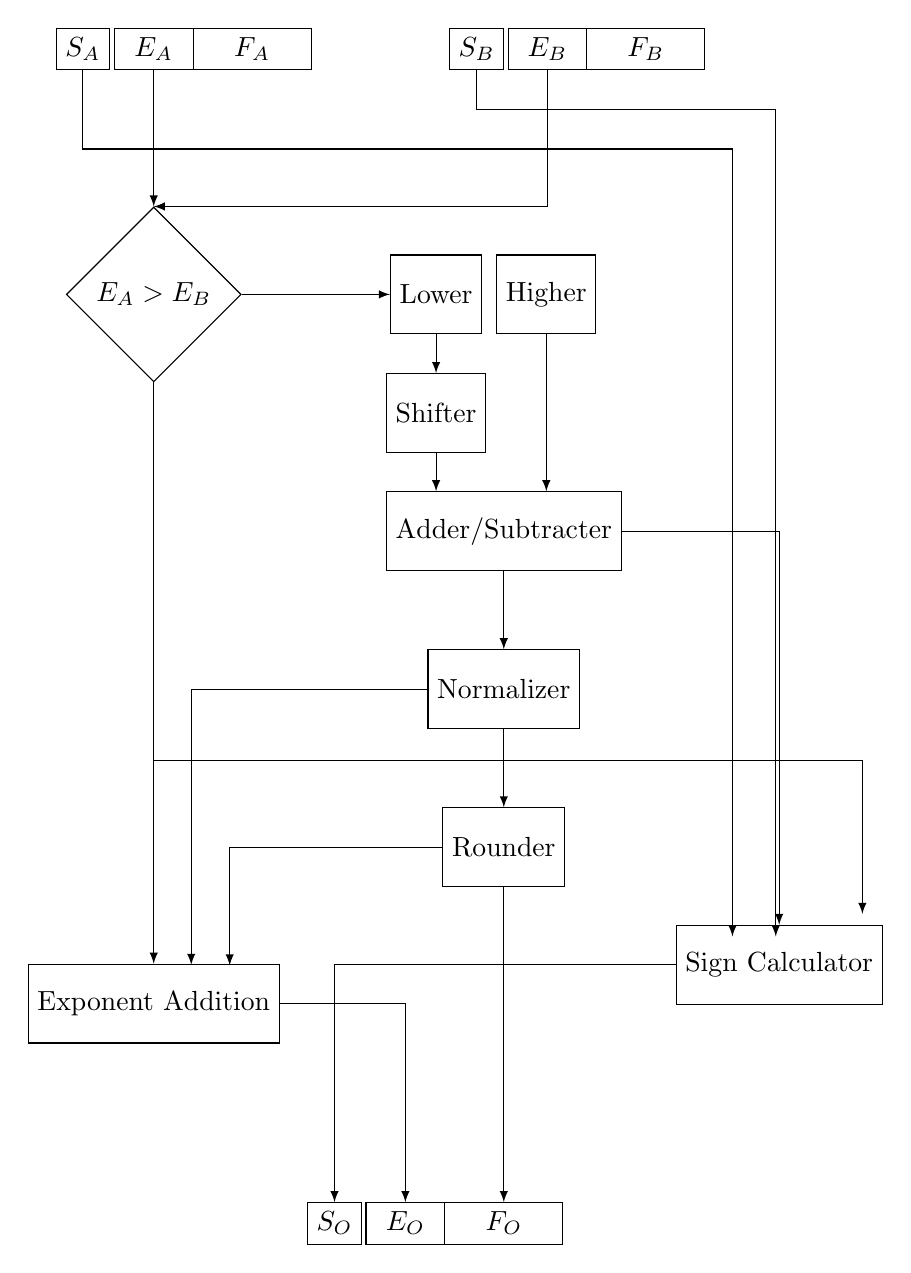
\begin{tikzpicture}
\node[draw,
        minimum width=0.6cm,
        minimum height=0.5cm] (SA) at (0,0) {$S_A$};
\node[draw,
        minimum width=1cm,
        minimum height=0.5cm] (EA) at ($(SA) + (.9, 0)$) {$E_A$};
\node[draw,
        minimum width=1.5cm,
        minimum height=0.5cm] (FA) at ($(EA) + (1.25, 0)$) {$F_A$};

\node[draw,
        minimum width=0.6cm,
        minimum height=0.5cm] (SB) at (5,0) {$S_B$};
\node[draw,
        minimum width=1cm,
        minimum height=0.5cm] (EB) at ($(SB) + (.9, 0)$) {$E_B$};
\node[draw,
        minimum width=1.5cm,
        minimum height=0.5cm] (FB) at ($(EB) + (1.25, 0)$) {$F_B$}; 

\draw [-latex]
    (EA) --++(0, -2) 
    node[diamond, draw, anchor=north] (comp) {$E_A>E_B$};

\draw [-latex]
    (EB) -- (EB |- comp.north) -- (comp.north);

\draw [-latex]
    (comp) --++(3, 0)
    node[draw, 
        minimum width=1cm,
        minimum height=1cm, anchor=west] (low) {Lower};

\node[draw, 
        minimum width=1cm,
        minimum height=1cm] (high) at ($(low) + (1.4, 0)$) {Higher};        

\draw [-latex]
    (low) --++(0, -1)
    node[draw, 
        minimum width=1cm,
        minimum height=1cm, anchor=north] (shift) {Shifter};

\node[draw,
        minimum width=1cm,
        minimum height=1cm,
        anchor=west] (add) at ($(shift.west) + (0, -1.5)$) {Adder/Subtracter};

\draw [-latex] 
    (shift) -- (shift |- add.north);

\draw [-latex]    
    (high) -- (high |- add.north);

\draw [-latex]
    (add) --++(0, -1.5)
     node[draw, 
        minimum width=1cm,
        minimum height=1cm, 
        anchor=north] (norm) {Normalizer};

\draw [-latex]
    (norm) --++(0, -1.5)
     node[draw, 
        minimum width=1cm,
        minimum height=1cm, 
        anchor=north] (Rou) {Rounder};

\draw [-latex]
    (comp) --++(0, -8.5)
     node[draw, 
        minimum width=1cm,
        minimum height=1cm, 
        anchor=north] (Eadd) {Exponent Addition};    

\draw [-latex]
    (Rou.west) --++(-2.7, 0) --++(0, -1.5);

\draw [-latex] 
    (norm.west) --++(-3, 0) --++(0, -3.5);

\draw [-latex]
    (add.east) --++ (2, 0) --++(0, -5) node[draw,
        minimum width=1cm,
        minimum height=1cm, anchor=north] (sign) {Sign Calculator};

\draw [-latex]
    (Rou.south) --++ (0, -4) node[draw,
        minimum width=1.5cm,
        minimum height=0.5cm, anchor=north] (FO) {$F_O$};

\node[draw,
        minimum width=1cm,
        minimum height=0.5cm] (EO) at ($(FO) + (-1.25, 0)$) {$E_O$};                 
        
\node[draw,
        minimum width=0.6cm,
        minimum height=0.5cm] (SO) at ($(EO) + (-0.9, 0)$) {$S_O$};

\draw [-latex]   
    (Eadd.east) -- (EO.north |- Eadd.east) -- (EO.north);

\draw [-latex]
    (SA.south) --++ (0, -1) --++ (8.25, 0) --++ (0, -10);

\draw [-latex]
    (SB.south) --++ (0, -0.5) --++ (3.8, 0) --++ (0, -10.5);

\draw [-latex]
    (comp.south) --++ (0, -4.8) --++ (9.0, 0) --++ (0, -1.95);

\draw [-latex]
    (sign.west) -- (SO.north |- sign.west) -- (SO.north);

\end{tikzpicture}
\caption{Flow chart of the addition/substraction algorithm}
\end{figure}

\newpage

\section{\large{High-level Block Diagram of the Architecture}}

\vspace{15mm}

\ctikzset{
    logic ports=ieee,
    logic ports/scale=1
}

\begin{figure}[H]
    \centering

\begin{circuitikz}

\tikzset{mux/.style={muxdemux,
 muxdemux def={Lh=6, NL=4, Rh=4, NT=2, NB=0, w=2.5, square pins=1}}}


\tikzset{adder/.style={muxdemux,
 muxdemux def={Lh=6, NL=2, Rh=6, NT=1,
 NB=1, w=3, square pins=1}}}

 \tikzset{box12/.style={muxdemux,
 muxdemux def={Lh=10, Rh=10, NL=1, NR=2, NT=2, NB=1, w=2, square pins=1}}}

 \tikzset{box11/.style={muxdemux,
 muxdemux def={Lh=5, Rh=5, NL=1, NR=1, NT=0, NB=0, w=2, square pins=1}}}

 \tikzset{box21/.style={muxdemux,
 muxdemux def={Lh=6, Rh=6, NL=2, NR=1, NT=0, NB=0, w=2, square pins=1}}}

 \tikzset{box31/.style={muxdemux,
 muxdemux def={Lh=15, Rh=15, NL=3, NR=1, NT=0, NB=0, w=2, square pins=1}}}

\node[box12, rotate=-90](added) at (0,0){\rotatebox{90}{Added Input}};
\draw[<-] (added.blpin 1) --++(0,3) node[above]{$ A $};
\draw[->] (added.rpin 2) --++(0,-2)
    node[box11, rotate=-90, anchor=blpin 1](expmod){\rotatebox{90}{Exp Modifier}};
\draw[->] (expmod.rpin 1) --++(0, -2)
    node[box31, rotate=-90, anchor=blpin 2](out){\rotatebox{90}{Output Process}};
\draw[->] (added.rpin 1) --++(0, -0.5)
    node[box11, rotate=-90, anchor=blpin 1](norm){\rotatebox{90}{Normalizer}};
\draw[->] (norm.rpin 1) --++(0, -1.5)
    node[box11, rotate=-90, anchor=blpin 1](round){\rotatebox{90}{Rounder}};
\draw[->] (round.rpin 1) -- (out.blpin 1);
\draw[->] (added.bpin 1) --(added.bpin 1 -| out.lpin 3) node[above]{sign}
    -- (out.blpin 3);
\node[box21, rotate=-90](inpchk) at (7,1.5){\rotatebox{90}{Input Checker}};
\draw[<-] (inpchk.blpin 1) --++(0, 1.5) node[above]{$ B $};
\draw[->] (inpchk.rpin 1) --++(0, -0.25)
    node[right]{\tiny{both input non-zero}} --++(0, -3)
    node[and port, anchor=bin 1, rotate=-90](and){};
\draw[->] (added.tpin 1) --++(2.5,0) node[above]{\tiny{Shifted non-zero}} --
    (added.tpin 1 -| and.in 2) -- (and.bin 2);
\draw[->] (out.rpin 1) --++(0, -1) --++(4, 0) --++(0, -1)
    node[mux, rotate=-90, anchor=blpin 3](mx){\rotatebox{90}{4$\times$1 MUX}};
\draw[<-] (mx.blpin 4) --++(0, 1);
\draw[<-] (inpchk.blpin 2) --++(0, 1) coordinate(a) -- (a -| added.lpin 1);
\draw[<-] (mx.blpin 2) -- (mx.blpin 2 |- a);
\draw[<-] (mx.blpin 1) --++(0, 12.25) coordinate(b) -- (b -| inpchk.lpin 1);
\draw[->] (and.out) -- (and.out |- mx.tpin 2) -- (mx.btpin 2);
\draw[<-] (mx.btpin 1) --++(1,0) coordinate(c) -- (c |- added.tpin 2) -- (added.btpin 2);
\draw[->] (mx.rpin 1) --++(0, -1) node[below]{Output};
\end{circuitikz}
 \caption{Block Diagram of FPA}
    \label{fig:block_diagram1}
\end{figure}

\begin{figure}[H]
    \centering

\begin{circuitikz}

\tikzset{mux/.style={muxdemux,
 muxdemux def={Lh=4, NL=2, Rh=3, NT=0, NB=1, w=2, square pins=1}}}

\tikzset{adder/.style={muxdemux,
 muxdemux def={Lh=6, NL=2, Rh=6, NT=1,
 NB=1, w=3, square pins=1}}}

 \tikzset{box12/.style={muxdemux,
 muxdemux def={Lh=10, Rh=10, NL=1, NR=2, NT=2, NB=1, w=2, square pins=1}}}

 \tikzset{box11/.style={muxdemux,
 muxdemux def={Lh=5, Rh=5, NL=1, NR=1, NT=0, NB=0, w=2, square pins=1}}}

  \tikzset{box11c/.style={muxdemux,
 muxdemux def={Lh=5, Rh=5, NL=1, NR=1, NT=1, NB=0, w=2, square pins=1}}}

  \tikzset{box11cc/.style={muxdemux,
 muxdemux def={Lh=5, Rh=5, NL=1, NR=1, NT=0, NB=1, w=2, square pins=1}}}

 \tikzset{box21/.style={muxdemux,
 muxdemux def={Lh=6, Rh=6, NL=2, NR=1, NT=1, NB=0, w=2, square pins=1}}}

  \tikzset{box21c/.style={muxdemux,
 muxdemux def={Lh=12, Rh=12, NL=2, NR=1, NT=0, NB=1, w=2, square pins=1}}}

 \tikzset{box41/.style={muxdemux,
 muxdemux def={Lh=8, Rh=8, NL=4, NR=1, NT=0, NB=0, w=2, square pins=1}}}


\node[box21, rotate=-90](comp) at (0,0){\rotatebox{90}{Comparision}};
\draw[<-] (comp.blpin 2) --++(0, 2) coordinate(x) node[above]{$A$};
\draw[->] (comp.brpin 1) --++(0, -2)
    node[box11c, rotate=-90, anchor=blpin 1](expdiff){\rotatebox{90}{Exp Diff}};
\draw[->] (comp.btpin 1) --++(6, 0) --++(0, -1.5) --++(0.5,0)
    node[mux, rotate=-90, anchor=bbpin 1](mx1){\rotatebox{90}{MUX}};

\draw[->] (mx1.rpin 1) --(mx1.rpin 1 |- expdiff.blpin 1)
    node[box11cc, rotate=-90, anchor=blpin 1](shifter){\rotatebox{90}{Shifter}};
\draw[->] (shifter.rpin 1) --++(0, -1)
    node[box21c, rotate=-90, anchor=blpin 2](as){\rotatebox{90}{Adder/Subtractor}};
\draw[<-] (as.blpin 1) -- (as.blpin 1 |- mx1.brpin 1)
    node[mux, rotate=-90, anchor=brpin 1](mx2){\rotatebox{90}{MUX}};
\draw[<-] (mx2.bbpin 1) --++(-0.5, 0) coordinate(a) --(a |- comp.tpin 1)
    -- (comp.tpin 1);
\draw[->] (as.bbpin 1) --++(-1, 0) --++(0, -1)
    node[box41, rotate=-90, anchor=blpin 1](sign){\rotatebox{90}{Sign Computation}};
\draw[<-] (mx2.blpin 1) -- (mx2.blpin 1 |- x) coordinate(y) node[above]{$ B $};
\draw[<-] (comp.blpin 1) --++(0, 0.75) coordinate(z) --(z -| y);
\draw[<-] (sign.blpin 3) -- (sign.blpin 3 |- z);
\draw[<-] (mx2.blpin 2) --++(0, 3) coordinate(c) -- (c -| comp.blpin 2);
\draw[<-] (sign.blpin 4) -- (sign.blpin 4 |- c);
\draw[<-] (sign.blpin 2) -- (sign.blpin 2 |- comp.tpin 1);
\draw[<-] (mx1.blpin 1) -- (mx1.blpin 1 |- z);
\draw[<-] (mx1.blpin 2) -- (mx1.blpin 2 |- c);

\draw[->] (expdiff.brpin 1) --++ (0, -5) coordinate(t) node[below]{exp};
\draw[->] (sign.brpin 1) -- (sign.brpin 1 |- t) node[below]{sign};
\draw[->] (as.brpin 1) -- (as.brpin 1 |- t) node[below]{sum};

\draw (sign.lpin 4) node[right]{\tiny{$A$}};
\draw (sign.lpin 3) node[right]{\tiny{$B$}};
\draw (sign.lpin 2) node[right]{\tiny{$A > B$}};
\draw (sign.lpin 1) node[right]{\tiny{$C_{out}$}};
\draw[->] (expdiff.btpin 1) -- (shifter.bbpin 1);

\end{circuitikz}
 \caption{Block Diagram of Added Input}
    \label{fig:block_diagram2}
\end{figure}

\begin{figure}[H]
    \centering

\begin{circuitikz}

\tikzset{mux/.style={muxdemux,
 muxdemux def={Lh=4, NL=2, Rh=3, NT=1, NB=0, w=2.5, square pins=1}}}

\node[xor port](xor1) at (0,0){};
\draw (xor1.out) --++(1, 0) node[and port, anchor=in 1](and1){};
\draw (and1.out) --++(1, 0) --++(0, -2) --++(0.5, 0) node[xor port, anchor=in 1](xor2){};
\draw (xor2.out) --++(1,0) node[mux, anchor=lpin 1](mux){MUX};
\draw (xor2.in 2) --++(-0.5, 0) --++(0, -2) --++(-1, 0) node[and port, anchor=out](and2){};
\draw (and2.in 2) --++(-1, 0) node[xor port, anchor=out](xor3){};
\draw (and1.in 2) --++(-0.5, 0) --++(0, -1) --++(-1, 0)
    node[not port, anchor=out](not){};
\draw (and2.in 1) --++(-0.15, 0) coordinate(a) --(a |- and1.in 1);
\draw (and1.in 1) --++(-0.5, 0) coordinate(a) --++(0, 0.5) coordinate(b)
    -- (b -| mux.tpin 1) -- (mux.tpin 1);
\draw (xor1.in 1) --++(-0.25, 0) coordinate(c) --++(-0.75, 0) node[left]{$A$};
\draw (xor1.in 2) --++(-1, 0) node[left]{$B$};
\draw (not.in) --++(-1, 0) node[left]{$C_{out}$};
\draw (mux.lpin 2) --(mux.lpin 2 -| c) -- (c);
\draw (xor3.in 1) --++(-0.5, 0) coordinate(d) -- (d |- xor1.in 2);
\draw (xor3.in 2) --++(-1, 0) node[left]{$ A > B $};
\draw (mux.rpin 1) --++(1, 0) node[right]{ sign };
\end{circuitikz}
 \caption{Block Diagram of Sign Computation}
    \label{fig:block_diagram3}
\end{figure}
\newpage

\section{\large{Comprehensive Design Description}}
\subsection{Comparing the Exponents and Aligning Radix Point}
To add two floating-point numbers, the radix points must be aligned. This is typically done by shifting the input with the smaller exponent to the right to align it with the larger input. We have used a comparator to compare the exponents of the two inputs and a 12-bit subtractor to calculate the difference between them.

\subsection{Shifting}
Multiplexer-based shifters have been used to perform all shifting operations. To obtain bit shifts of any arbitrary amount up to 31, we have used five 32-bit multiplexers. The multiplexers can shift respectively 1, 2, 4, 8 and 16 bits. Combining them, we can get any number of shifts up to 31, as is shown in \ref{fig:arbleftshift} and \ref{fig:arbrightshift}. In case of aligning two fractions, we may need more than 31 shifts which result in all bits being 0. Moreover, the input to the shifter circuit should be the difference of the exponents. Therefore, the lower 5 bits are be used for shifting when all the upper 7 bits are clear. Only in that case, the shift amount does not exceed 31($2^{5}-1$). Otherwise, the fraction will be 0(all bits cleared), which is done in \ref{fig:rightshiftwithempty}.

\subsection{Normalization}
In order to normalize followed by addition operation, we employed a priority encoder to identify the position of the most significant set bit, which is the leftmost one. Four 8 to 1 priority encoders are used to implement this. 
The result can be upto 31($0_{th} to 31_{th}$), hence consisting of 5 bits($0-2^{5}-1$). Output of the encoders are lower 3 bits of the result. Upper two bit and outputs of the encoders are selected using their valid bits. If left most encoder gets a valid input, other encoders will not be selected and upper two bits will be 00. So the range of the numbers generated will be from 0 to 7 in decimal. Similarly, when the second encoder is selected upper two bits will be 01; 10 and 11 for third and fourth ones respectively. The selection bit of the multiplexer is passed from a 4 to 2 priority encoder whose inputs are the valid bits of the aforementioned priority encoders. If inputs to neither of the priority encoders are valid, it means the fraction contains only 0s. This can happen in two cases.
\begin{enumerate}
    \item The result is of the structure $1.00 * 2^{x}$
    \item The result is $0.0$
\end{enumerate}
The first case can appear if two numbers of type $1.00 * 2^{x-1}$ and equal exponents are added. So, we can check whether the signs of both input are same. If they are, we will continue the algorithm and increase the exponent by 1. If the signs are opposite, the result is actually 0. So, output is 0.0.

\subsection{Rounding}
In order to add and subtract the mantissas, we employed a 32-bit adder. However, we can only retain 19 bits, so we may need to round the result in some instances. We consider $20th$ bit as Guard bit, $21th$ as Round bit. If any of the bits on the right of Round bit is set, Sticky bit will be set. Otherwise, it is clear. We need to consider these cases:\\
\begin{center}
\begin{tabular}{|c|c|c|c|c|}
    \hline
    \textbf{$19th$ bit} & \textbf{G} & \textbf{R} & \textbf{S} & \textbf{Action}  \\
    \hline
    X & 0 & X & X & Truncate \\
    \hline
    1 & 1 & X & X & Round up \\
    \hline
    0 & 1 & 0 & 0 & Truncate \\
    \hline 
    X & 1 & 1 & X & Round up \\
    \hline 
    X & 1 & X & 1 & Round up \\
    \hline
\end{tabular}
\end{center}
Actually X100 is the case for round to even. So, if 19th bit is 0, we need to do nothing, hence truncation. Otherwise, we will round up. For simplification we will use K-map. ($19th bit = M$) 
\begin{center}
\begin{karnaugh-map}[4][4][1][S][R][G][M]
    \minterms{5, 6, 7, 12, 13, 14, 15}
    \maxterms{1, 2, 3, 4, 8, 9, 10, 11}
    \implicant{5}{15}
    \implicant{7}{14}
    \implicant{12}{14}
\end{karnaugh-map}
\end{center}
\[ flag = GS + GR + MG = G(M + R + S) \]
If flag is set, 1 is added at the $19th$ position. Otherwise, the bits beyond the 20th position are truncated.

\subsection{Computing the Sign Bit}
There are certain considerations to take into account when calculating the sign bit. If the signs of the two inputs are the same, then the sign of the output will be either of the signs of the inputs.
If they are not the same, we have to consider two things. Firstly, we need to find the sign of the output of the adder. It can be calculated using the equation:
\begin{equation}
sign = (S_A \oplus S_B)\overline{C_{out}}
\label{eq1}
\end{equation}
Where $C_{out}$ is the carry out of the adder.
However, this sign may not always be correct because we always subtract the input with the smaller exponent from the input with the higher exponent. When the signs of the inputs are opposite, i.e, if the input with greater exponent is negative and the other one is positive, \ref{eq1} gives opposite to the correct. To fix this we have introduced a variable switch. This switch bit will alter the sign bit in those cases. Our sign bit will fail when the sign bits of inputs are opposite and the input with greater exponent is negative. In that case switch will become 1 and will alter the sign. Equation of switch bit is:
\begin{equation}
switch = (S_A \oplus S_B)(Comp \oplus S_B)
\label{eq2}
\end{equation}
Here, Comp is the output of the comparator circuit($Exp_{A} > Exp_{B}$). So, the formula for sign bit:
\begin{equation}
actualSign = sign \oplus switch 
\label{eq3}
\end{equation}
Equation \ref{eq3} will be used in case the signs of the inputs are different. Otherwise, The sign of the first input will be directly applied to the sign of the output. This selection will be made using a multiplexer.

\subsection{Handling Zero or Small Input}
\label{zero}
If either of the inputs is zero, the other input will be passed directly to the output. Additionally, if the exponent of one of the inputs is significantly smaller than the other (a difference of more than 31), the input with the larger exponent is passed directly to the output.

\subsection{Increasing Precision}
\label{incprec}
For addition, we did not set aside a bit to capture the overflow bit. Instead, we captured the bit directly from the carry out. Besides, in case of subtraction, we did not use a separate bit for the sign. Instead, the carry out of the adder was used to determine the sign of the result. If the carry out is 1, the result of subtraction is positive, otherwise negative. It is an exception when one of the summands is zero. Therefore, this case was handled separately as stated in \ref{zero}. As a result, the precision is increased by 2.

\newpage

\section{\large{ICs Used with Count as a Chart}}
\begin{table}[H]
    \centering
    \begin{tabular}{lc}
         \textbf{IC} & \textbf{Quantity}  \\
         \hline
         \hline
            IC 7404 & 2 \\
            IC 7408 & 10 \\
            IC 7432 & 46 \\ 
            IC 7483 & 41 \\
            IC 7485 & 3 \\
            IC 7486 & 25 \\ 
            IC 74147 & 5 \\ 
            IC 74157 & 205 \\
         \hline
         Total & 337  \\
    \end{tabular}
    \caption{ICs Used with Quantity}
    \label{tab:ic_quantity}
\end{table}
\newpage

\section{\large{Simulator used Along with the Version Number}}
Logisim 2.16.1.4 has been used for simulating the floating point adder circuit.

\section{\large{Discussion}}
In this assignment, we put a concerted effort to ensure the novelty and utmost efficiency of the design. In a lot of instances, we took the difficult route of implementing the modules by ourselves or coining an algorithm just to avoid using additional bits. This might have cost us huge efforts, but we ended up achieving a design we can claim to be as novel as it can get. \\
\newline
As explained in \ref{incprec}, we did not reserve a separate bit for capturing overflow or the sign of the result. This allowed us to improve the precision of our implementation by 2 digits. However, it took some time to come up with the proper algorithm to correctly compute the result. We utilized the carry out from the adder to work around this limitation of no extra bit.\\
\newline
We also put a great deal of effort into fine-tuning our design and thoroughly testing it. To be absolutely spot on with our testing, we wrote a \href{https://github.com/risenfromashes/cse306/blob/master/FPA/Tester/FPA.cpp}{C++ program} to mimic our algorithm and then match its outputs with the ones of the adder. In several stages, it helped us rectify parts of our algorithm.\\
\newline
In addition to the technical aspects of our implementation, we also took great care to ensure the self-contained nature of our floating point adder. That is to say, rather than relying on external libraries, we implemented all the modular components of our adder by ourselves. This not only allowed us to fully understand the inner workings of our tool, but also made it more reliable and easy to maintain. From shifting bits using multiplexer to finding the leftmost set bit using priority encoders, we did it all. \\
\newline
Interestingly, this did pose a challenge at one point. As part of the report, we are expected to count the number of different ICs used in the design. But because we did so many abstractions, it was virtually impossible to count the number by hand. Module A might contain three instances of module C, module C might again contain two B’s, another module D might comprise of A’s, it is a humongous task to keep this track manually. We revisited the famous Depth First Search (DFS) algorithm to solve this problem. We constructed a graph considering the modules as vertices and their inter-dependencies as edges, and ran the DFS algorithm on it. This was another interesting bit of this assignment, that we really enjoyed doing. The source code can be found \href{https://github.com/risenfromashes/cse306/blob/master/FPA/Tester/ic_counter.cc}{here}. \\
\newline
Overall, the design and implementation of the floating point adder was an interesting task and we learned many new things along the way.\\
\end{document}
